\section{Introduction}

Mobile apps are utilized for virtually all aspects of daily life in the modern world. So after we noticed that there is no application that allows the efficient planning of campaigns like the "Sternsinger-Aktion", we asked ourselves why, and furthermore, how hard it is to create an app with intuitive usability with the main purpose of simplifying the process of managing such a campaign and gaining a general overview of the progress made by the groups.

\blankLine

The app needs to comply with specific criteria we defined in cooperation with Prof. DI Robert Müllerferli. He is the main organizer of the campaign in the parish of Lieboch and helped us to work out the key aspects our project should implement. In the finished product, every user should be able to scan a QR-Code, through which the area of this group gets assigned to the device. These areas must be dynamically adjustable, so an admin can coordinate the workload of each area more efficiently. The areas also need to be clearly visible by an outline that gets drawn through "Border" addresses. We implement an algorithm to calculate these border addresses. It should be visible at a glance if there is a "specification", which can be assigned by admins and set for an address. We should achieve this by employing distinct icons rather than the default one. Apart from the app itself, we also implemented a web portal through which administrators can manage and supervise the campaign. 

\blankLine

The investigative aspect of this thesis will focus on how components should behave and appear, so that new users can use this tool without requiring a long "onboarding" phase. Interacting with elements should feel familiar, and the limits of what users can and cannot do need to be clearly defined. Our application needs a reliable data source to ensure the consistency and accuracy of marked addresses, so we researched ways to keep our database up to date with minimal manual intervention. After defining the project requirements, we identified a need to determine which addresses qualify as border addresses. 

In our context, an area consists of multiple addresses, each with a defined location represented by latitude and longitude coordinates. Border addresses are the ones that form the outer boundary of an area. For example, given five addresses with the following coordinates:


    \begin{itemize}
        \setstretch{1}
        \item A (0,0)
        \item B (2,0)
        \item C (0,2)
        \item D (-2,0)
        \item E (0,-2)
    \end{itemize}


In this case, addresses B, C, D, and E are border addresses because they outline the area, enclosing A at the center.
 Thus, we explored different algorithms for this task, compared them in terms of efficiency, selected the most suitable one, and implemented it.

\blankLine

This thesis contains an in-depth description of our thought and development process, as well as the steps we took to achieve our goal of a functional mobile application that can be used by volunteers during the "Sternsinger-Aktion 2025," which took place in the parish of Lieboch in January 2025.

\blankLine

The result of this thesis should be a mobile app that provides users with the addresses that they need to visit on this day. They then should be able to easily mark the houses they already visited. If something unusual occurs at this address, the user should be able to record it, ensuring that the organizers are aware of it and can account for it in the future.

\newpage

\subsection{Team}

\begin{figure}[H]
        \centering
        \begin{minipage}{0.6\textwidth}
          \setlength{\baselineskip}{1.5em}
          \vspace{-1em}
          \textbf{Leon Edlinger}

          The Admin Panel was developed by Leon. He researched how adaptive algorithms and real-time data integration can be used to continuously update address databases and ensure accuracy in an app designed for mobile response teams. 
        \end{minipage}
        \hfill
        \begin{minipage}{0.35\textwidth}
            \center
            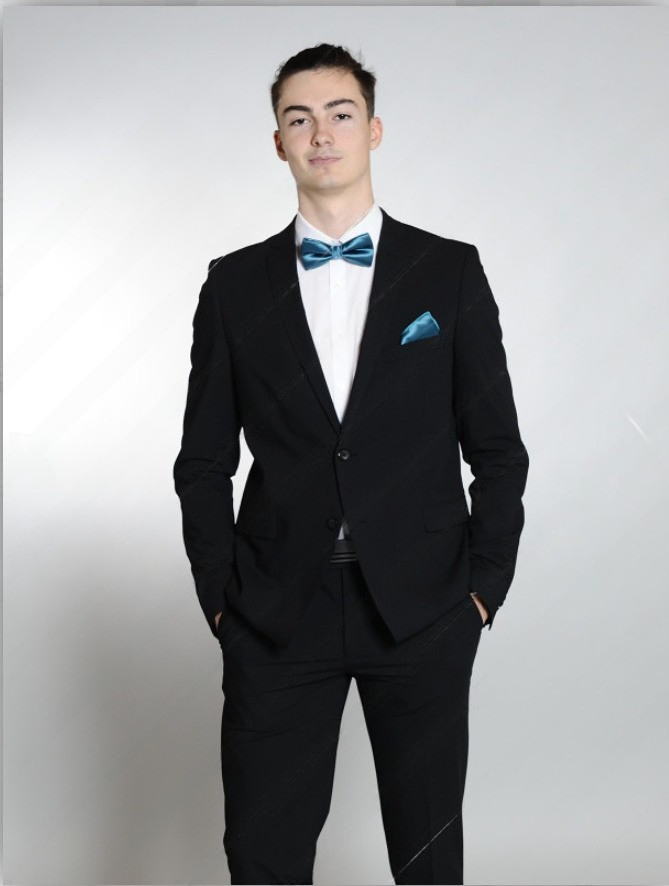
\includegraphics[width=0.8\textwidth]{images/people/leonEdlinger.jpeg} 
    \end{minipage}
    \end{figure}

    \begin{figure}[H]
        \centering
        \begin{minipage}{0.35\textwidth}
            \center
            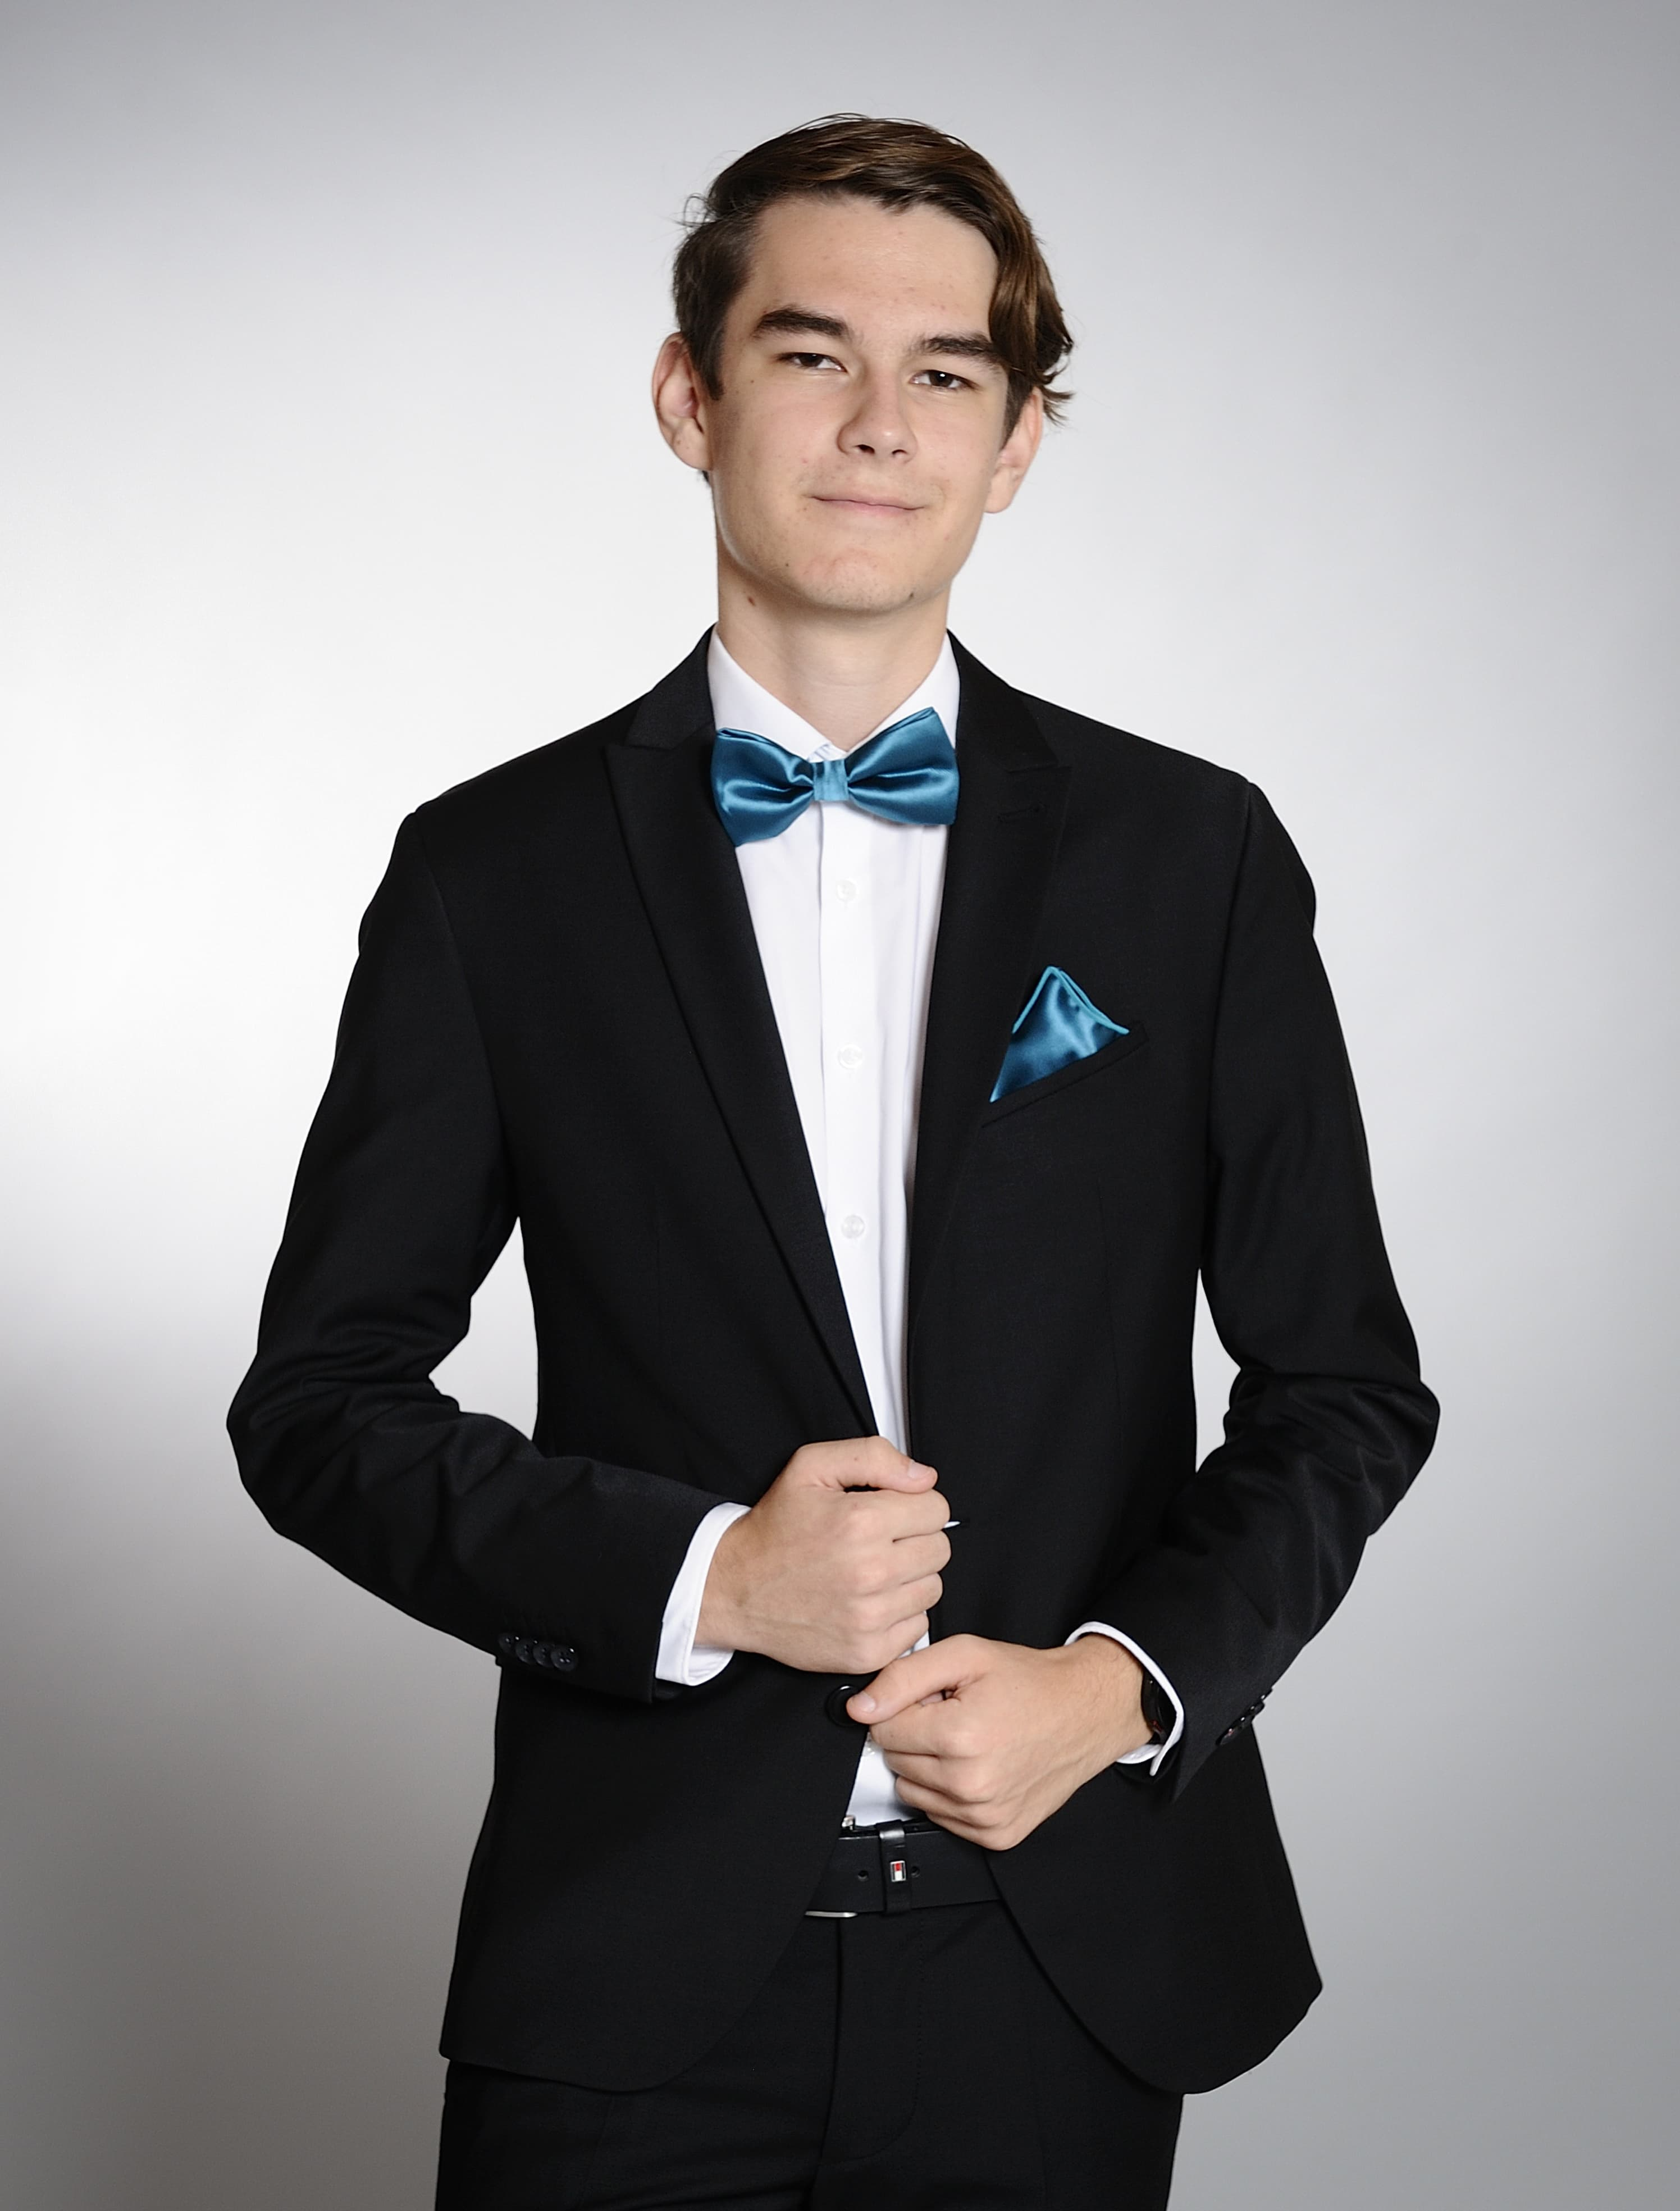
\includegraphics[width=0.8\textwidth]{images/people/paulGigler.jpeg} 
    \end{minipage}
    \hfill
        \begin{minipage}{0.6\textwidth}
          \setlength{\baselineskip}{1.5em}
          \vspace{-1em}
          \textbf{Paul Gigler}

          Paul designed and developed the mobile application and was responsible for the deployment of our software. Additionally, he acted as the team-leader and was responsible for maintaining the contact with the end users. He researched on how user experience principles can contribute to an intuitive map display for charitable activities involving people with different technical expertise.
        \end{minipage}
    \end{figure}

    \begin{figure}[H]
        \centering
        \begin{minipage}{0.6\textwidth}
          \setlength{\baselineskip}{1.5em}
          \vspace{-1em}
          \textbf{Andreas Weissl}

          The task of Andreas was developing the backend server. He researched how modern algorithms for geodata analysis and route optimization can be used to improve the efficiency and coverage of the area distribution in the caroling campaign.
        \end{minipage}
        \hfill
        \begin{minipage}{0.35\textwidth}
            \center
            
\includegraphics[width=0.8\textwidth]{images/people/andreasWeissl.jpeg}
    \end{minipage}
    \end{figure}

\newpage